\subsection{Aeronautics \& Quaternions}
Aeronautics often deal with the problem of rotation.
An airplane has an ``internial frame", which needs to be corresponded to the `` body frame."
A common way to represent rotation on an airplane is with the following convention:
\begin{figure}[H]
\centering
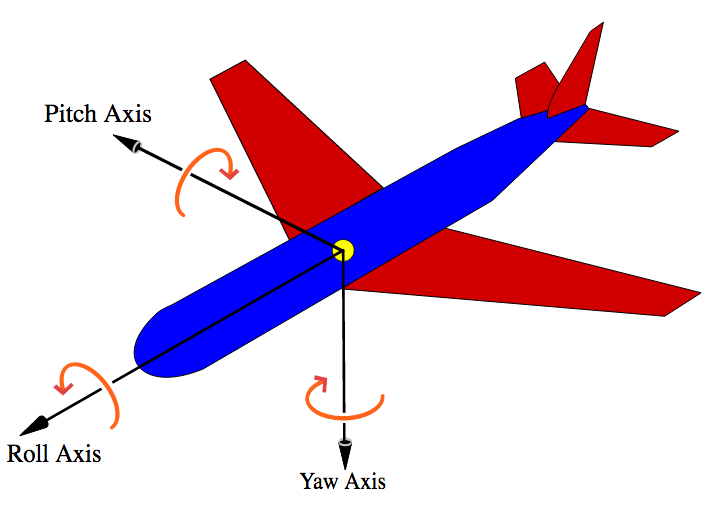
\includegraphics[width = .75\textwidth]{Figures/plane.png}
\caption{Roll, Pitch, and Yaw}
\label{fig:cycle}
\end{figure}
Roll, pitch, and yaw are simply Euler angles.
When flying a small plane, and rotating about a single axis, it may be easier to use Euler angles.
However, many large commerical airlines use computer assisted flight with many maneuvers done on autopilot.
Complicated rotations may be represented as an arbitrary rotation about an arbitrary axis, the perfect use case for quaternions.


\subsection{Computer Graphics \& Quaternions}
